\documentclass[14pt]{extbook}
\usepackage{multicol, enumerate, enumitem, hyperref, color, soul, setspace, parskip, fancyhdr} %General Packages
\usepackage{amssymb, amsthm, amsmath, bbm, latexsym, units, mathtools} %Math Packages
\everymath{\displaystyle} %All math in Display Style
% Packages with additional options
\usepackage[headsep=0.5cm,headheight=12pt, left=1 in,right= 1 in,top= 1 in,bottom= 1 in]{geometry}
\usepackage[usenames,dvipsnames]{xcolor}
\usepackage{dashrule}  % Package to use the command below to create lines between items
\newcommand{\litem}[1]{\item#1\hspace*{-1cm}\rule{\textwidth}{0.4pt}}
\pagestyle{fancy}
\lhead{Progress Quiz 5}
\chead{}
\rhead{Version B}
\lfoot{9912-2038}
\cfoot{}
\rfoot{Spring 2021}
\begin{document}

\begin{enumerate}
\litem{
Factor the quadratic below. Then, choose the intervals that contain the constants in the form $(ax+b)(cx+d); b \leq d.$\[ 24x^{2} -50 x + 25 \]\begin{enumerate}[label=\Alph*.]
\item \( a \in [0.27, 1.15], \hspace*{5mm} b \in [-30, -25], \hspace*{5mm} c \in [0.97, 1.27], \text{ and } \hspace*{5mm} d \in [-20, -18] \)
\item \( a \in [2.93, 3.48], \hspace*{5mm} b \in [-5, -3], \hspace*{5mm} c \in [6.6, 10.14], \text{ and } \hspace*{5mm} d \in [-7, -2] \)
\item \( a \in [11.17, 13.83], \hspace*{5mm} b \in [-5, -3], \hspace*{5mm} c \in [1.68, 2.07], \text{ and } \hspace*{5mm} d \in [-7, -2] \)
\item \( a \in [5.38, 7.01], \hspace*{5mm} b \in [-5, -3], \hspace*{5mm} c \in [3.48, 4.82], \text{ and } \hspace*{5mm} d \in [-7, -2] \)
\item \( \text{None of the above.} \)

\end{enumerate} }
\litem{
Factor the quadratic below. Then, choose the intervals that contain the constants in the form $(ax+b)(cx+d); b \leq d.$\[ 36x^{2} +60 x + 25 \]\begin{enumerate}[label=\Alph*.]
\item \( a \in [0.8, 1.1], \hspace*{5mm} b \in [30, 32], \hspace*{5mm} c \in [0.3, 1.9], \text{ and } \hspace*{5mm} d \in [26, 33] \)
\item \( a \in [1.9, 4.8], \hspace*{5mm} b \in [3, 8], \hspace*{5mm} c \in [10.4, 14.9], \text{ and } \hspace*{5mm} d \in [-3, 6] \)
\item \( a \in [5.3, 7.9], \hspace*{5mm} b \in [3, 8], \hspace*{5mm} c \in [5.1, 6.9], \text{ and } \hspace*{5mm} d \in [-3, 6] \)
\item \( a \in [11.3, 12.9], \hspace*{5mm} b \in [3, 8], \hspace*{5mm} c \in [2.4, 5.4], \text{ and } \hspace*{5mm} d \in [-3, 6] \)
\item \( \text{None of the above.} \)

\end{enumerate} }
\litem{
Write the equation of the graph presented below in the form $f(x)=ax^2+bx+c$, assuming  $a=1$ or $a=-1$. Then, choose the intervals that $a, b,$ and $c$ belong to.
\begin{center}
    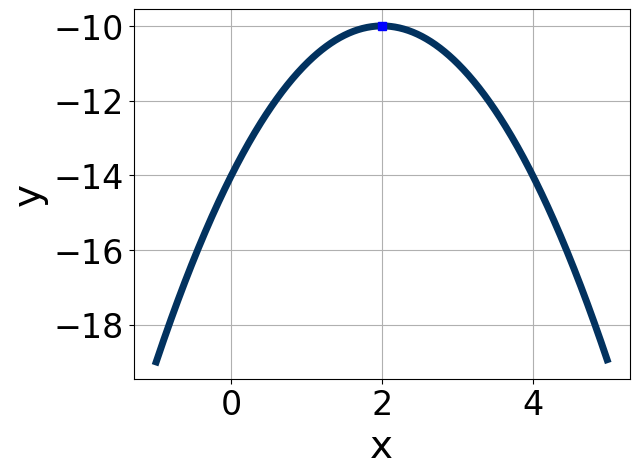
\includegraphics[width=0.5\textwidth]{../Figures/quadraticGraphToEquationB.png}
\end{center}
\begin{enumerate}[label=\Alph*.]
\item \( a \in [-1.4, 0.1], \hspace*{5mm} b \in [2, 5], \text{ and } \hspace*{5mm} c \in [-9, -6] \)
\item \( a \in [0.7, 1.2], \hspace*{5mm} b \in [-4, 1], \text{ and } \hspace*{5mm} c \in [-2, 1] \)
\item \( a \in [0.7, 1.2], \hspace*{5mm} b \in [-4, 1], \text{ and } \hspace*{5mm} c \in [7, 12] \)
\item \( a \in [0.7, 1.2], \hspace*{5mm} b \in [2, 5], \text{ and } \hspace*{5mm} c \in [-2, 1] \)
\item \( a \in [-1.4, 0.1], \hspace*{5mm} b \in [-4, 1], \text{ and } \hspace*{5mm} c \in [-9, -6] \)

\end{enumerate} }
\litem{
Graph the equation below.\[ f(x) = (x+4)^2 - 20 \]\begin{enumerate}[label=\Alph*.]
\begin{multicols}{2}\item 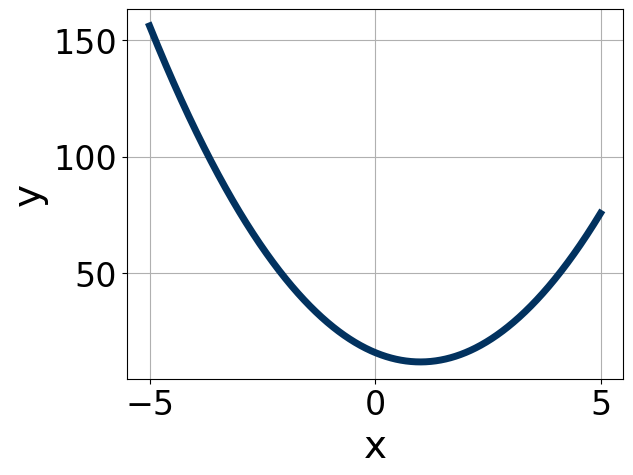
\includegraphics[width = 0.3\textwidth]{../Figures/quadraticEquationToGraphAB.png}\item 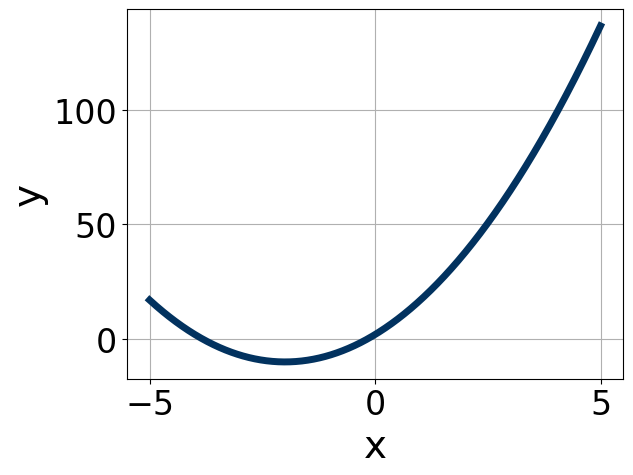
\includegraphics[width = 0.3\textwidth]{../Figures/quadraticEquationToGraphBB.png}\item 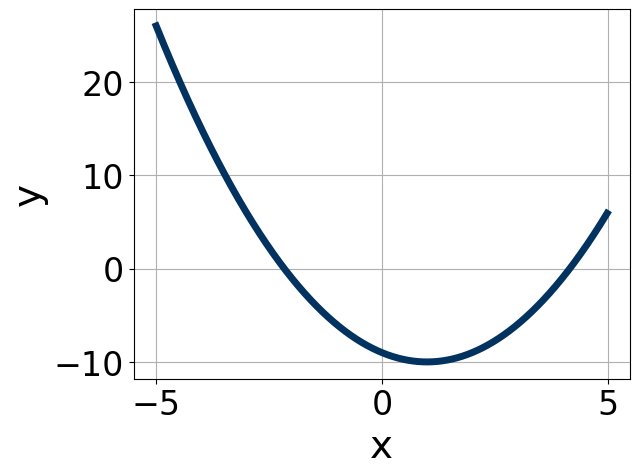
\includegraphics[width = 0.3\textwidth]{../Figures/quadraticEquationToGraphCB.png}\item 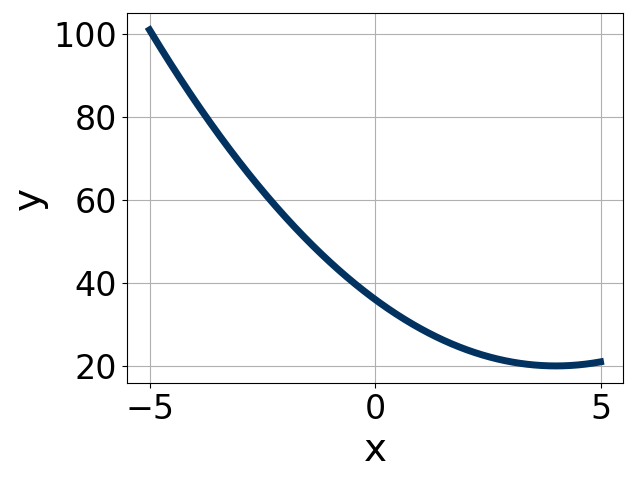
\includegraphics[width = 0.3\textwidth]{../Figures/quadraticEquationToGraphDB.png}\end{multicols}\item None of the above.
\end{enumerate} }
\litem{
Solve the quadratic equation below. Then, choose the intervals that the solutions $x_1$ and $x_2$ belong to, with $x_1 \leq x_2$.\[ 25x^{2} -10 x -24 = 0 \]\begin{enumerate}[label=\Alph*.]
\item \( x_1 \in [-0.46, -0.33] \text{ and } x_2 \in [2.32, 2.44] \)
\item \( x_1 \in [-4.16, -3.87] \text{ and } x_2 \in [0.16, 0.35] \)
\item \( x_1 \in [-20.02, -19.95] \text{ and } x_2 \in [29.99, 30.09] \)
\item \( x_1 \in [-1.22, -0.45] \text{ and } x_2 \in [1.04, 1.28] \)
\item \( x_1 \in [-2.58, -2.18] \text{ and } x_2 \in [0.34, 0.41] \)

\end{enumerate} }
\litem{
Solve the quadratic equation below. Then, choose the intervals that the solutions belong to, with $x_1 \leq x_2$ (if they exist).\[ 18x^{2} +11 x -5 = 0 \]\begin{enumerate}[label=\Alph*.]
\item \( x_1 \in [-22.86, -21.28] \text{ and } x_2 \in [20.6, 24] \)
\item \( x_1 \in [-1.63, -0.7] \text{ and } x_2 \in [-0.2, 0.9] \)
\item \( x_1 \in [-16.69, -16.24] \text{ and } x_2 \in [4.3, 6.1] \)
\item \( x_1 \in [-0.52, -0.05] \text{ and } x_2 \in [0.4, 1.9] \)
\item \( \text{There are no Real solutions.} \)

\end{enumerate} }
\litem{
Solve the quadratic equation below. Then, choose the intervals that the solutions $x_1$ and $x_2$ belong to, with $x_1 \leq x_2$.\[ 25x^{2} +10 x -24 = 0 \]\begin{enumerate}[label=\Alph*.]
\item \( x_1 \in [-3.65, -3.51] \text{ and } x_2 \in [0.21, 0.42] \)
\item \( x_1 \in [-0.63, 0.05] \text{ and } x_2 \in [1.36, 1.79] \)
\item \( x_1 \in [-30.25, -29.65] \text{ and } x_2 \in [19.96, 20.2] \)
\item \( x_1 \in [-1.49, -0.78] \text{ and } x_2 \in [0.64, 0.9] \)
\item \( x_1 \in [-6.28, -5.58] \text{ and } x_2 \in [-0.07, 0.23] \)

\end{enumerate} }
\litem{
Write the equation of the graph presented below in the form $f(x)=ax^2+bx+c$, assuming  $a=1$ or $a=-1$. Then, choose the intervals that $a, b,$ and $c$ belong to.
\begin{center}
    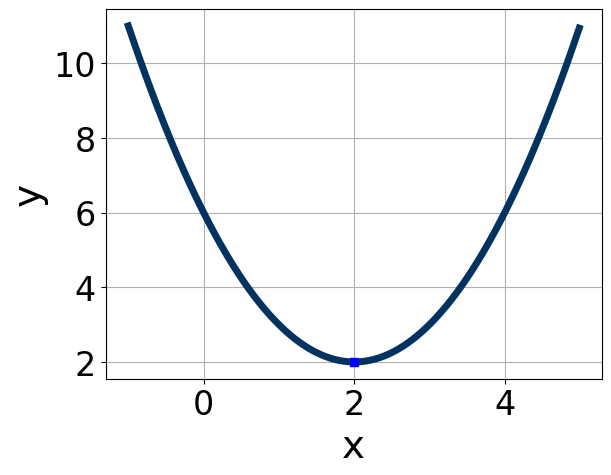
\includegraphics[width=0.5\textwidth]{../Figures/quadraticGraphToEquationCopyB.png}
\end{center}
\begin{enumerate}[label=\Alph*.]
\item \( a \in [-4, 0], \hspace*{5mm} b \in [-6, -1], \text{ and } \hspace*{5mm} c \in [-4, 1] \)
\item \( a \in [-4, 0], \hspace*{5mm} b \in [-6, -1], \text{ and } \hspace*{5mm} c \in [-8, -5] \)
\item \( a \in [-4, 0], \hspace*{5mm} b \in [4, 5], \text{ and } \hspace*{5mm} c \in [-8, -5] \)
\item \( a \in [1, 3], \hspace*{5mm} b \in [-6, -1], \text{ and } \hspace*{5mm} c \in [0, 5] \)
\item \( a \in [1, 3], \hspace*{5mm} b \in [4, 5], \text{ and } \hspace*{5mm} c \in [0, 5] \)

\end{enumerate} }
\litem{
Solve the quadratic equation below. Then, choose the intervals that the solutions belong to, with $x_1 \leq x_2$ (if they exist).\[ -11x^{2} -15 x + 8 = 0 \]\begin{enumerate}[label=\Alph*.]
\item \( x_1 \in [-4, -1.1] \text{ and } x_2 \in [0.1, 1.6] \)
\item \( x_1 \in [-25.1, -24] \text{ and } x_2 \in [22.8, 26.2] \)
\item \( x_1 \in [-4.9, -4.1] \text{ and } x_2 \in [18.4, 20] \)
\item \( x_1 \in [-0.7, 2] \text{ and } x_2 \in [1, 2.1] \)
\item \( \text{There are no Real solutions.} \)

\end{enumerate} }
\litem{
Graph the equation below.\[ f(x) = (x-3)^2 + 13 \]\begin{enumerate}[label=\Alph*.]
\begin{multicols}{2}\item 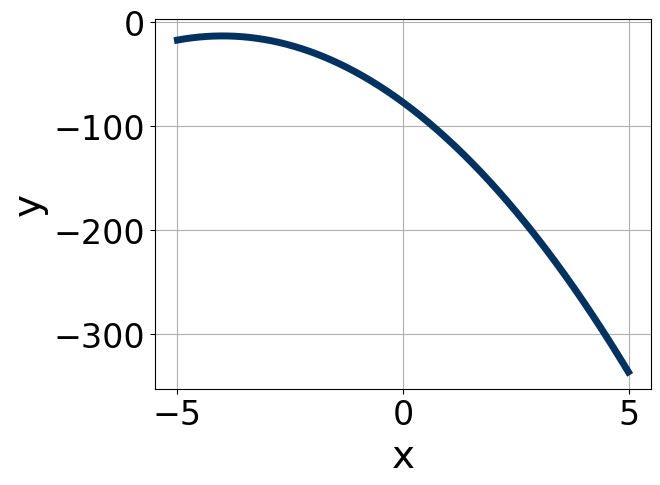
\includegraphics[width = 0.3\textwidth]{../Figures/quadraticEquationToGraphCopyAB.png}\item 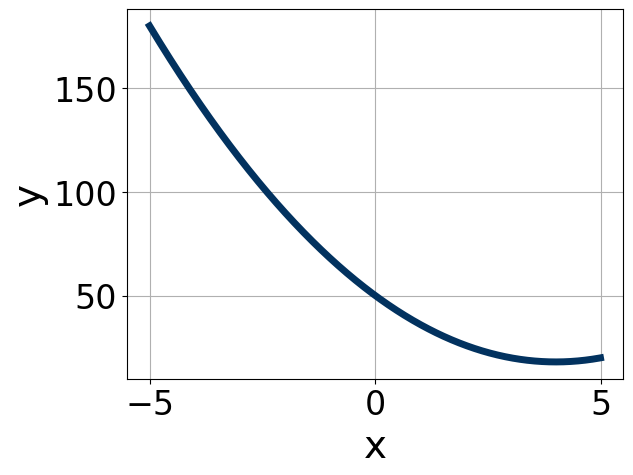
\includegraphics[width = 0.3\textwidth]{../Figures/quadraticEquationToGraphCopyBB.png}\item 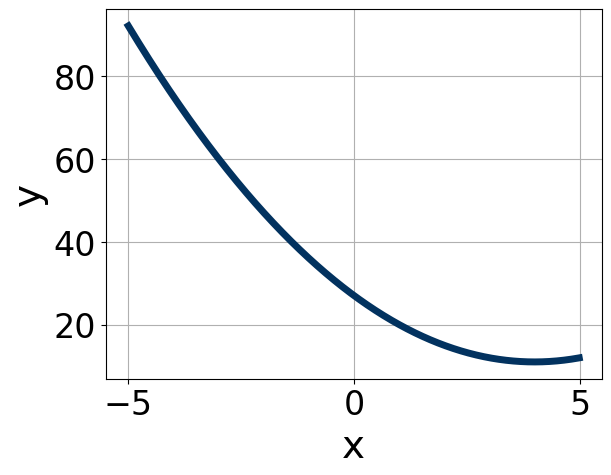
\includegraphics[width = 0.3\textwidth]{../Figures/quadraticEquationToGraphCopyCB.png}\item 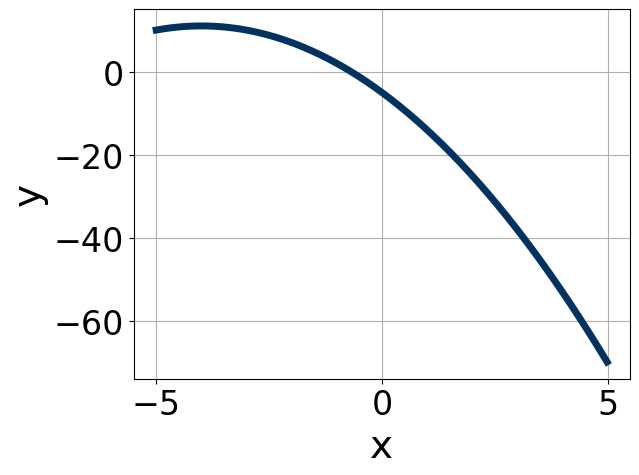
\includegraphics[width = 0.3\textwidth]{../Figures/quadraticEquationToGraphCopyDB.png}\end{multicols}\item None of the above.
\end{enumerate} }
\end{enumerate}

\end{document}